\documentclass[11pt]{article}

\usepackage[T1]{fontenc}
\usepackage[utf8]{inputenc}
\usepackage{amsmath,amssymb}
\usepackage{booktabs}
\usepackage{tabularx}
\usepackage{longtable}
\usepackage{geometry}
\usepackage[hidelinks]{hyperref}
\usepackage[numbers]{natbib}
\usepackage{microtype}
\usepackage{seqsplit}
\usepackage{tikz}
\usetikzlibrary{arrows.meta,positioning,shapes.geometric,fit}
\geometry{margin=1in}
\setlength{\emergencystretch}{3em}

\newcommand{\RaS}{Repository-as-State}
\newcommand{\RRI}{Repository Resumability Index}
\newcommand{\RTF}{Reconstruction Token Fraction}
\newcommand{\breakcode}[1]{\texttt{\seqsplit{#1}}}
\newcommand{\mixedstatus}{\texttt{MIXED\_\allowbreak METHODOLOGY\_\allowbreak AND\_\allowbreak MODEL\_\allowbreak FAILURE}}

\title{Repository-as-State:\\Externalising Agent Continuity for Stateless High-Capability Reasoning}
\author{Paul Maddison\\Independent Researcher\\Liverpool, United Kingdom}
\date{Paper v1.0 --- research-programme release --- 6 September 2026}

\begin{document}
\maketitle

\begin{abstract}
Long-horizon software-engineering agents can retain conversational history, summaries, memory stores, execution state, and repository observations across tasks. This paper asks whether one part of that continuity---predecessor high-capability reasoning-session history---is necessary after a software-engineering transition has reached an accepted durable state. \emph{Repository-as-State} (RaS) treats accepted project state as the persistent programme object and compares persistent-session continuation with fresh-session reconstruction under matched task, model/runtime, workspace and verification controls. Here ``stateless'' refers only to predecessor reasoning-session continuity; durable repository state and controlled execution state are not removed.

The contribution is deliberately narrower than repository-aware coding, Git-backed memory, durable workflow execution, or sequential software-agent evaluation, all of which have substantial prior art. RaS focuses on disposal at \emph{accepted engineering boundaries}, where the predecessor's decision-relevant consequences should already have been externalised into project artefacts, and treats reconstruction cost as a separate falsification route rather than assuming it is free.

The empirical record is bounded and mixed. The original P0 methodology pilot was executed once and classified \mixedstatus; its A/B correctness outcome is not treated as causal evidence. Subject-B P1 observed 18/30 behaviours in each condition with 30/30 matched behaviour agreements. Subject-B P2 observed 0/39 in each condition with 39/39 agreements, a floor effect that provides no positive evidence of successful behavioural preservation. One independent Subject-C cross-repository replication step observed 12/30 behaviours for persistent-session A and 15/30 for fresh-session B, with 25/30 matched agreements, five disagreements (one favouring A and four B), and candidate full passes tied at 2/9 per condition. The task-solving model is stochastic, Subject C has only three repetitions per task, and its 30 behaviour observations are nested within nine matched task-by-repetition experimental units; the observed direction is therefore descriptive only, not evidence of systematic superiority, equivalence, or non-inferiority. P1, P2 and Subject C are not pooled.

These results do not establish that conversation context never matters, that repository state is universally sufficient, or that RaS is cheaper or more secure. They support a narrower conclusion: the post-acceptance value of predecessor reasoning state is an experimentally tractable systems question, and authoritative repository state can be evaluated as a continuity boundary without treating accumulated conversation as project state.
\end{abstract}

\noindent\textbf{Keywords:} software engineering; AI coding agents; agent continuity; repository state; reproducibility; empirical software engineering.

\section{Introduction}
\label{sec:introduction}

Software-engineering agents increasingly operate across repositories, shells, test runners, browsers, issue trackers, build systems, and other development tools. SWE-bench established repository-level issue resolution as a measurable software-engineering task \citep{jimenez2024swebench}; SWE-agent showed that the design of the agent--computer interface materially affects navigation, editing, and testing \citep{yang2024sweagent}; and OpenHands provides an open platform and SDK for software agents with sandboxed execution, lifecycle control, memory management, and model routing \citep{wang2024openhands,wang2025openhandsSDK}. Sequential evaluation is also no longer novel in itself: SWE-STEPS evaluates coding agents across chains of dependent pull requests and shows that isolated-task success can hide spillover effects \citep{shastry2026swesteps}.

Agent memory is likewise an active research area. MemGPT manages information across memory tiers \citep{packer2023memgpt}; recent surveys cover episodic, semantic, reflective, hierarchical, and learned memory mechanisms \citep{du2026memory,luo2026memory}; and repository-specific work uses commit history or Git-bound ledgers as agent memory \citep{wang2025repomemory,li2026learningcommit,guo2026gitmemory}. RaS therefore cannot claim novelty for repository-aware agents, external memory, Git-backed memory, repository retrieval, or sequential coding evaluation.

The narrower question is architectural and causal:

\begin{quote}
\textbf{After an engineering transition has been accepted and its consequences persisted, how much additional value does predecessor reasoning-session state provide for the next dependent task?}
\end{quote}

RaS investigates the hypothesis that, for a meaningful class of sequential software-engineering work, accepted project state can carry enough decision-relevant continuity that the high-capability reasoning process does not need to persist between accepted transitions. The central proposition remains:

\begin{quote}
\textbf{Durable engineering continuity does not necessarily need to live inside the expensive high-capability reasoning process.}
\end{quote}

This is not the claim that reasoning disappears as a computational cost. A fresh reasoner may need to rediscover information, and that rediscovery can dominate the workload. Indeed, Handoff Debt finds that when coding tasks are interrupted mid-work, repository-only takeover requires substantially more events and prompt tokens than context-bearing handoffs, while solve-rate effects are smaller and model dependent \citep{kc2026handoff}. That evidence is adverse to any naive claim that repository-only resumption is automatically efficient. RaS therefore places its reset boundary after \emph{validated accepted transitions}, not at arbitrary interruption points, and treats reconstruction cost as a first-class possible falsifier.

The central inversion can still be stated compactly:

\begin{quote}
\textbf{The persistent object need not be the developer; it can be the software.}
\end{quote}

Software projects offer unusually rich domain-native durable state: source code, tests, schemas, build definitions, architecture records, Git history, configuration, and validation evidence. Engineers have always externalised decisions into such artefacts. That practice is not the novelty. The RaS question is what this existing property implies for the lifecycle of expensive reasoning processes.

We define a reasoning process as \emph{disposable with respect to programme continuity} when terminating and replacing it after an accepted engineering transition does not materially reduce subsequent correct continuation, provided that the replacement receives the same authoritative durable state and current task and is matched on model capability/configuration, tool interface, and execution environment. The definition is behavioural. It does not assert that the replacement reproduces the predecessor's internal reasoning or that no recomputation occurs. The current experiments do not establish this property generally; they provide bounded samples against it.

Figure~\ref{fig:ras-architecture} summarises the proposed loop.

\begin{figure}[htbp]
\centering
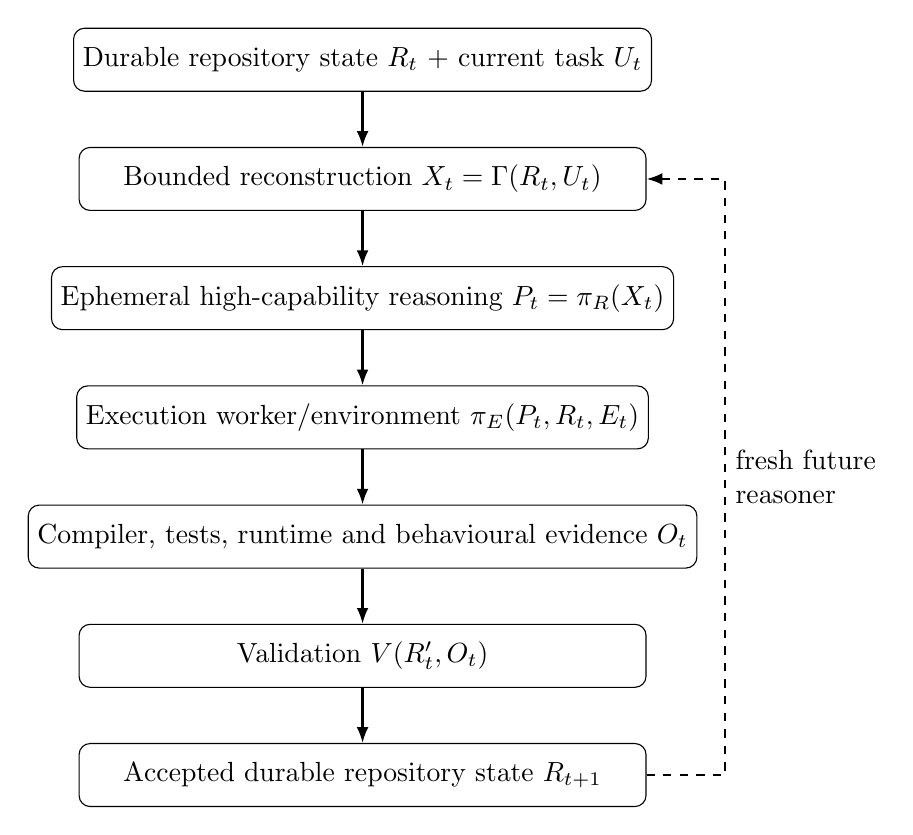
\begin{tikzpicture}[
node distance=7mm,
box/.style={draw,rounded corners,align=center,minimum width=7.2cm,minimum height=8mm},
arrow/.style={-{Latex[length=2mm]},thick}
]
\node[box] (state) {Durable repository state $R_t$ + current task $U_t$};
\node[box,below=of state] (recon) {Bounded reconstruction $X_t=\Gamma(R_t,U_t)$};
\node[box,below=of recon] (reason) {Ephemeral high-capability reasoning $P_t=\pi_R(X_t)$};
\node[box,below=of reason] (exec) {Execution worker/environment $\pi_E(P_t,R_t,E_t)$};
\node[box,below=of exec] (evidence) {Compiler, tests, runtime and behavioural evidence $O_t$};
\node[box,below=of evidence] (validate) {Validation $V(R'_t,O_t)$};
\node[box,below=of validate] (next) {Accepted durable repository state $R_{t+1}$};
\draw[arrow] (state)--(recon);
\draw[arrow] (recon)--(reason);
\draw[arrow] (reason)--(exec);
\draw[arrow] (exec)--(evidence);
\draw[arrow] (evidence)--(validate);
\draw[arrow] (validate)--(next);
\draw[arrow,dashed] (next.east) -- ++(1.0,0) |- node[pos=0.25,right,align=left]{fresh future\\reasoner} (recon.east);
\end{tikzpicture}

\caption{Conceptual Repository-as-State architecture. The durable object is accepted project state; reasoning and execution processes may be replaced between validated transitions. The figure is architectural, not empirical evidence.}
\label{fig:ras-architecture}
\end{figure}

The architecture is:
\[
R_t + U_t
\rightarrow
\text{bounded reconstruction}
\rightarrow
\text{high-capability reasoning}
\rightarrow
\text{execution}
\rightarrow
\text{validation}
\rightarrow
R_{t+1}.
\]
After acceptance, the reasoning process may be terminated. A later fresh process reconstructs what it needs from $R_{t+1}$ and the next task.

The idea arose from repeated practical workflows involving human problem selection, high-capability AI reasoning, bounded implementation packages, local execution agents, deterministic evidence, repository persistence, and fresh reasoning sessions. That origin is \textbf{OBSERVED MOTIVATION}. It is vulnerable to confirmation bias, author familiarity, survivor bias, and undocumented human assistance, and it is not experimental validation.

After hostile review of current prior work, this paper claims the following narrower contributions:

\begin{enumerate}
    \item a post-acceptance \emph{reasoning-state disposal} hypothesis for sequential software engineering, distinguished from interrupted-task handoff and Git-bound transcript memory;
    \item a matched persistent-history versus forced-reset experimental intervention intended to vary predecessor conversational/model-native history while holding accepted repository state, task, model, tools, and environment constant;
    \item a bounded empirical application of that intervention across the methodology-corrected P1/P2 studies and one independent cross-repository Subject-C replication step, reported without pooling or post-hoc equivalence claims;
    \item an explicit \emph{measurement design}, not an executed outcome claim, for repository rediscovery and structured non-chain-of-thought state-reconstruction probes as possible falsification routes when fresh-session reconstruction is costly or incomplete;
    \item a broader lifecycle framing in which reasoning persistence, execution state, and operational privilege can be varied independently, while treating semantic-state ablation, tiered execution, reconstruction economics, and security benefits as future or secondary hypotheses rather than findings of the accepted outcome set.
\end{enumerate}

The empirical record is now bounded rather than absent. P0 was executed once and rejected for causal A/B correctness interpretation after a mixed methodology/model failure. P1 observed equal non-zero behavioural performance in its three-task sample; P2 observed equal floor-level performance in a four-task, three-repetition same-repository block; and Subject C added one independent cross-repository replication step with mostly matched outcomes plus five discordant behaviour observations. Because the task-solving model is stochastic, the samples are small, Subject C has only nine matched task-by-repetition units, and no equivalence/non-inferiority design was preregistered, none of these results establishes general disposability, superiority, equivalence, or universal repository-state sufficiency.

\section{The Agent Continuity Problem}
\label{sec:continuity-problem}

Long-running software-engineering work is path dependent. A later task may depend on an earlier architectural decision, interface, regression test, migration, or failure mode. A future actor must recover enough relevant state to continue correctly.

Agentic systems can accumulate conversational history, tool observations, repository exploration, build results, hypotheses, rejected approaches, environment state, retry history, model outputs, and task progress. Persistent systems may preserve conversation, compacted context, summaries, episodic memory, working memory, server-side state, cached prompts, or persistent tool sessions. These mechanisms can be useful and are not claimed to be unnecessary.

Memory systems such as MemGPT manage information across tiers \citep{packer2023memgpt}; current surveys cover a broad family of persistent and retrieved agent memories \citep{du2026memory,luo2026memory}. Repository-specific memory work also uses commit history and Git-bound session artefacts \citep{wang2025repomemory,guo2026gitmemory}. The RaS question is therefore not whether memory exists, but where the \emph{marginal continuity value} lies after an engineering transition has been accepted.

Software engineering is an unusually favourable domain because project state can include:
\begin{itemize}
    \item source and generated interfaces;
    \item tests and behavioural constraints;
    \item Git history and accepted diffs;
    \item configuration/toolchain definitions;
    \item schemas and migrations;
    \item architecture/security records;
    \item product/behavioural documentation;
    \item CI/build evidence.
\end{itemize}

Let $H_t$ denote \emph{predecessor reasoning-session history not already represented as allowed project state}, $R_t$ the accepted project/repository state, $U_t$ the next task, and $S$ verifier-defined success. Conceptually, the continuity hypothesis asks whether:
\begin{equation}
P(S\mid R_t,U_t)
\approx
P(S\mid H_t,R_t,U_t)
\label{eq:continuity}
\end{equation}
over a declared task/model/environment population.

This is not the P0 estimator. Section~\ref{sec:sufficiency} defines the observable matched A/B target. The equation only states what marginal information $H_t$ is supposed to represent.

The hypothesis is plausible because engineering decisions are routinely reified, but that practice is not novel and does not prove sufficiency. Important rationale can remain outside the repository; documentation can be stale; tests can be incomplete; external systems can contain authoritative runtime facts. A repository may be excellent at preserving one task's constraints and poor at another's.

Conversation history also contains guesses, abandoned hypotheses, and stale observations. Repository artefacts can likewise be wrong, but many can be independently checked by compilers, tests, schemas, build systems, and behavioural verification. This motivates the research principle:
\begin{quote}
\textbf{Persist authoritative state. Reconstruct computation.}
\end{quote}

The principle is a hypothesis about engineering lifecycle boundaries, not a general law of agents.

\section{Repository-as-State}
\label{sec:ras}

RaS models an engineering programme as a sequence of validated transitions over durable repository state. The notation distinguishes durable state, active reasoning context, reasoning, execution, observations, and acceptance.

Let:
\begin{itemize}
    \item $R_t$ be the durable repository state at time $t$;
    \item $U_t$ be the current engineering task;
    \item $H_t$ be accumulated conversational or agent history;
    \item $Q_t$ be the high-capability reasoning process;
    \item $E_t$ be the execution worker and environment;
    \item $O_t$ be deterministic or runtime observations produced during execution.
\end{itemize}

A reconstruction function $\Gamma$ constructs the active reasoning view:
\begin{equation}
X_t = \Gamma(R_t,U_t).
\label{eq:gamma}
\end{equation}
The high-capability reasoner applies a reasoning policy $\pi_R$:
\begin{equation}
P_t = \pi_R(X_t),
\label{eq:reason}
\end{equation}
where $P_t$ is a bounded engineering proposal, transition plan, or work package.

Execution applies the proposal against current repository state in environment $E_t$:
\begin{equation}
(R'_t,O_t)=\pi_E(P_t,R_t,E_t).
\label{eq:execute}
\end{equation}
A validation function decides whether the candidate state is acceptable:
\begin{equation}
V(R'_t,O_t)\in\{0,1\}.
\label{eq:validate}
\end{equation}
If $V=1$, the durable state advances:
\begin{equation}
R_{t+1}=\mathrm{Commit}(R'_t).
\label{eq:commit}
\end{equation}
If validation fails, the candidate must not silently become authoritative. The protocol may permit repair within the current transaction, escalation, or a recorded failure, but the accepted repository state remains unchanged until the acceptance rule is satisfied.

After Equation~\ref{eq:commit}, $Q_t$ may be destroyed. A future process $Q_{t+1}$ should, under the strong RaS hypothesis, be able to operate from
\begin{equation}
R_{t+1}+U_{t+1}
\end{equation}
without requiring the complete $H_t$ that produced earlier transitions.

This model makes three separations explicit.

\subsection{Durable state versus active context}

Repository-as-State is not Repository-as-Prompt. A repository can contain millions of tokens, generated artefacts, vendored dependencies, long histories, and files irrelevant to the current task. Equation~\ref{eq:gamma} therefore matters as much as persistence itself. $R_t$ is the durable state space; $X_t$ is a selected reasoning view over that state.

The reconstruction function may use file search, symbol navigation, dependency tracing, test discovery, recent history, architecture records, build metadata, static analysis, or model-guided retrieval. It may also discover that a task requires information not durably represented in the repository. Such a discovery is evidence about repository sufficiency, not merely a retrieval inconvenience.

\subsection{Proposal versus execution}

$P_t$ is intentionally separated from $\pi_E$. A high-capability reasoner can propose a transition without necessarily possessing repository write access, shell access, cloud credentials, or unrestricted Git permissions. The executor may be cheaper, more stateful, more local, or simply more tightly sandboxed. RaS continuity does not depend on tiered execution, but the architecture makes tiering possible.

\subsection{Observation versus authority}

Tool output and model statements are not automatically authoritative. Compilation results, tests, runtime measurements, hidden behavioural verification, linters, and other observations enter $O_t$, but acceptance is represented separately by $V$. This matters because an agent can incorrectly state that a task is complete. A repository becomes a continuity substrate only to the extent that its transitions are governed by evidence.

Table~\ref{tab:state-artifacts} lists candidate durable-state carriers.

\begin{table}[htbp]
\centering
\small
\caption{Candidate durable state carriers in a Repository-as-State system.}
\label{tab:state-artifacts}
\begin{tabularx}{\textwidth}{@{}lX X@{}}
\toprule
Artefact & Continuity carried & Failure mode if absent or stale \\
\midrule
Source & Current implementation and interfaces & Behaviour must be rediscovered or inferred incorrectly \\
Tests & Executable behavioural constraints & Regressions and hidden invariants may be missed \\
Schemas/migrations & Data contracts and transition state & Compatibility or migration phase can be misread \\
Build/configuration & Reproducible environment assumptions & Fresh workers cannot reproduce evidence \\
Architecture records & Rationale and non-obvious boundaries & Rejected or unsafe designs may reappear \\
Git history & Accepted transitions and provenance & Prior intent and change sequence become harder to inspect \\
CI/runtime evidence & Verified properties of a state & Agent self-report can be mistaken for proof \\
\bottomrule
\end{tabularx}
\end{table}


The strongest version of RaS would exhibit three properties simultaneously: high engineering success after complete reasoning-state reset, bounded or slowly growing reconstruction cost, and no material loss in engineering quality relative to a persistent control. Those properties are not assumed. The experimental programme is designed to determine where they hold and where they fail.

\section{Externalising Engineering Continuity}
\label{sec:externalising}

Software engineering already externalises reasoning into durable artefacts. That is established practice, not a RaS contribution. Source code, regression tests, schemas, architecture records, configuration, and commit history all preserve consequences of earlier decisions. The RaS hypothesis concerns what this ordinary engineering property may permit at the \emph{agent lifecycle} level.

An engineering episode can contain false hypotheses, debugging attempts, discarded implementations, and repeated discussion. Once a task is accepted, the durable state may contain only a smaller set of decision-relevant consequences:
\[
\text{transient reasoning}
\rightarrow
\{\text{accepted implementation, tests, rationale, schemas, constraints}\}.
\]
This paper calls that \emph{decision-relevant semantic compression} only as descriptive terminology. It does not claim to have invented the engineering practice of persisting decisions in code, tests, and documentation.

The compression can be lossy. Final code may reveal what was done without explaining why; tests may omit intent; comments can become stale; rejected alternatives may matter later. Repository memory research explicitly exploits commit history to recover project-specific knowledge that snapshots omit \citep{wang2025repomemory,li2026learningcommit}, and Git-bound agent memory can persist session-derived rationale in addition to project artefacts \citep{guo2026gitmemory}. These are direct warnings against assuming that accepted source state is self-explanatory.

RaS therefore asks a narrower question: after an accepted transition, has enough decision-relevant state been externalised into the \emph{allowed project state} that predecessor reasoning-session history adds little marginal value for the next dependent task?

The allowed project state may include source, tests, schemas, build information, documentation, architecture records, and Git history available at the cutoff. It need not be a source snapshot alone. Conversely, it must not contain hidden copies of predecessor model transcripts unless the experimental condition explicitly treats those as a repository memory artefact.

If forced-reset agents fail because crucial rationale was not externalised, that is evidence against the strong repository-continuity hypothesis for that task. If semantic-state ablation removes an artefact class and success or reconstruction quality degrades, that suggests marginal continuity value. If an ablation has no effect, the information may be redundant or irrelevant.

The goal is not to celebrate externalisation. It is to identify whether accepted engineering artefacts can serve as a sufficiently strong recovery boundary for fresh high-capability reasoning and how much rediscovery that boundary imposes.

\section{From Stateful Agents to Transactional High-Capability Reasoning}
\label{sec:transactional}

RaS treats a high-capability reasoning episode as a bounded computation over externally persisted engineering state:
\begin{equation}
R_t + U_t
\rightarrow
\text{reasoning episode}
\rightarrow
\text{validated state transition}
\rightarrow
R_{t+1}.
\end{equation}
After $R_{t+1}$ is accepted, the reasoning process may be terminated and replaced.

The term \emph{transactional} is retained only as a lifecycle analogy. It does not imply ACID semantics, serialisability, transactional memory, deterministic replay, or database atomicity. Recent work on semantic isolation for durable AI workflows uses transaction terminology for a different problem: maintaining compatible semantic resources across paused and resumed workflows \citep{mozafari2026semantic}. RaS therefore uses “reasoning transaction” narrowly to mean a bounded reasoning episode over externally persisted authoritative state whose process identity need not survive after an accepted transition.

\subsection{Disposable reasoning is recomputation-tolerant, not computation-free}

A reasoning process is \emph{disposable with respect to programme continuity} if replacing it after an accepted transition does not materially impair the next correct programme continuation under a prespecified behavioural comparison, given matched durable state, task, model capability/configuration, tool interface, and execution environment.

This definition explicitly allows recomputation. A fresh reasoner may re-read files, rediscover dependencies, or re-establish architectural understanding. If that work is large, disposal may be technically feasible but economically inferior. “Disposable” therefore concerns lifecycle dependence, not elimination of reasoning cost.

Figure~\ref{fig:lifecycle} contrasts the persistent-history control with the forced-reset lifecycle.

\begin{figure}[htbp]
\centering
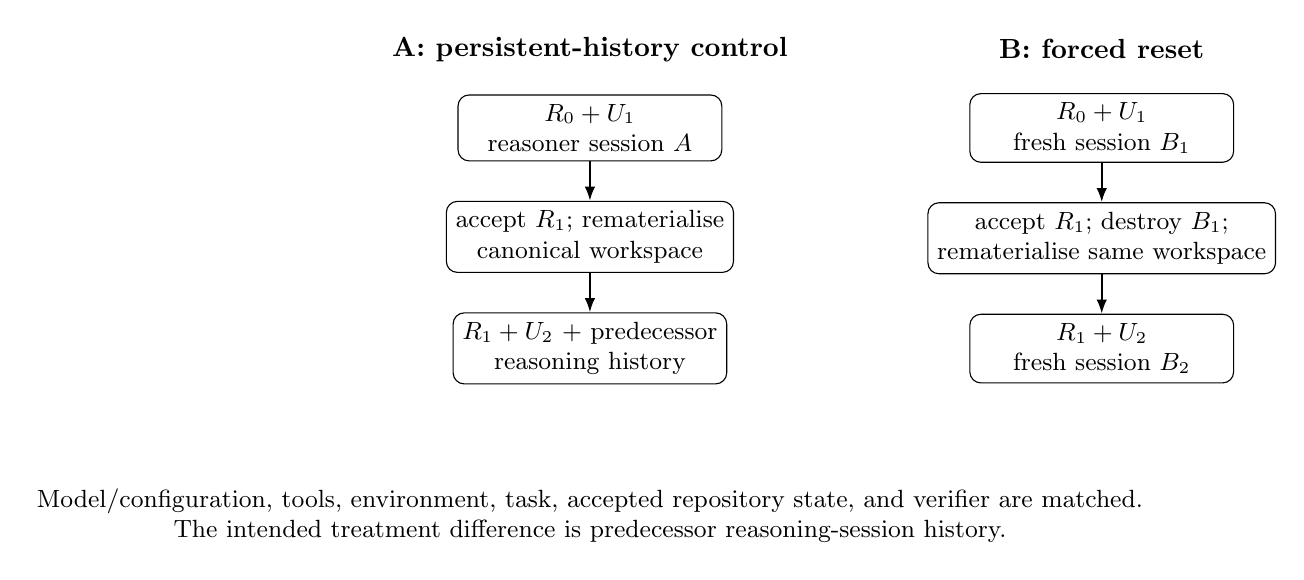
\begin{tikzpicture}[
node distance=5mm,
box/.style={draw,rounded corners,align=center,minimum width=3.35cm,minimum height=7mm,font=\small},
arrow/.style={-{Latex[length=1.8mm]},thick}
]
\node[font=\bfseries] at (-3.25,1.0) {A: persistent-history control};
\node[box] (p1) at (-3.25,0) {$R_0+U_1$\\reasoner session $A$};
\node[box,below=of p1] (p2) {accept $R_1$; rematerialise\\canonical workspace};
\node[box,below=of p2] (p3) {$R_1+U_2$ + predecessor\\reasoning history};
\draw[arrow] (p1)--(p2);
\draw[arrow] (p2)--(p3);

\node[font=\bfseries] at (3.25,1.0) {B: forced reset};
\node[box] (r1) at (3.25,0) {$R_0+U_1$\\fresh session $B_1$};
\node[box,below=of r1] (reset1) {accept $R_1$; destroy $B_1$;\\rematerialise same workspace};
\node[box,below=of reset1] (r2) {$R_1+U_2$\\fresh session $B_2$};
\draw[arrow] (r1)--(reset1);
\draw[arrow] (reset1)--(r2);

\node[below=12mm of p3,align=center,font=\small] (note) {Model/configuration, tools, environment, task, accepted repository state, and verifier are matched.\\The intended treatment difference is predecessor reasoning-session history.};
\end{tikzpicture}

\caption{Conceptual lifecycle comparison. The experimental treatment is predecessor reasoning-session history at an accepted engineering boundary; workspace, model, tools, task, and accepted repository state must otherwise be matched.}
\label{fig:lifecycle}
\end{figure}

Checkpoint/restart and stateless-service systems are important precedents rather than novelty claims. Durable Functions, for example, demonstrates reliable workflow execution with persisted state and reconstructable compute \citep{burckhardt2021durable}. Git already provides checkpoint-like accepted repository states. The RaS-specific question is semantic: whether those accepted software artefacts contain enough information that a fresh high-capability reasoner can continue a \emph{dependent engineering programme} without predecessor conversational/model-native history.

Potential properties such as restartability, horizontal scheduling, model routing, and lower session affinity are architectural implications only. Model routing is established prior work \citep{ong2024routellm}; cross-model continuity is not tested in P0 and remains future work.

The architecture also exposes failure classes. A reset run can fail because reconstruction selected the wrong evidence; because the reasoner misinterpreted correct evidence; because the proposal omitted a constraint; because execution failed; because the environment changed; or because validation was invalid. These mechanisms must not be collapsed into one causal explanation.

The central experimental requirement is therefore stronger than “open a new chat”. The audit requires canonical workspace rematerialisation and invariant system instructions, model configuration, task specification, tool interface, dependency state, and environment across conditions. If hidden provider/session memory or uncontrolled tool state differs between A and B, the treatment is not identifiable.

\section{Behavioural Repository Sufficiency}
\label{sec:sufficiency}

The original v0.1 draft expressed repository sufficiency through equality of latent distributions over “useful next actions” and a KL-divergence bound. Hostile review rejects that formulation for the experiments reported here. The action space is open-ended, equivalent implementations need not have comparable surface actions, and the runs do not expose a well-defined probability distribution over engineering actions. KL divergence would therefore add mathematical appearance without an estimable quantity.

The paper instead defines an observable behavioural target.

Let $Y_{s,d,c}\in\{0,1\}$ denote preregistered verifier-defined success for task sequence $s$, depth $d$, and condition $c$. Let $c=A$ be the persistent-history control and $c=B$ the forced-reset condition. The two conditions must use the same accepted starting repository state, current task, high-capability model/configuration, tool contract, workspace image, and acceptance criteria. The intended treatment difference is availability of predecessor reasoning-session history.

For a future repeated confirmatory experiment, define:
\begin{equation}
p_c(d)=P(Y=1\mid c,d,\mathcal{M},\mathcal{E},\mathcal{T}),
\label{eq:behavioural-success}
\end{equation}
where $\mathcal{M}$ identifies the matched model/configuration, $\mathcal{E}$ the controlled execution environment, and $\mathcal{T}$ the declared task-sampling population.

A future confirmatory study can preregister a scientifically justified non-inferiority margin $\delta>0$ and ask whether:
\begin{equation}
p_B(d)-p_A(d) \ge -\delta
\label{eq:noninferiority-target}
\end{equation}
over the declared task population and depth range. If symmetric equivalence is scientifically required, a two-sided margin can be preregistered instead. The margin must be fixed before outcomes and justified in engineering terms; the present programme does not invent one after seeing results.

P0 was a methodology pilot and cannot support such inference. P1, P2 and Subject C are likewise reported as bounded samples rather than confirmatory distributional estimates. Subject C has only three repetitions per task and nine matched task-by-repetition units. Its 30 behaviour observations are nested within those experimental units and within task contracts; they are not 30 independent replicates.

“Repository sufficiency” is therefore shorthand for a conditional behavioural hypothesis, not an intrinsic property of a repository. A repository may be adequate for one task class, model, tool interface, and depth but not another. It also need not preserve every past thought. The question is whether accepted durable state permits matched fresh reasoning to achieve useful engineering outcomes at acceptable reconstruction cost for a declared population.

Operational evidence can include:
\begin{itemize}
    \item verifier-defined task and behaviour outcomes;
    \item complete-sequence success across dependent tasks;
    \item success by sequential depth;
    \item reconstruction-probe accuracy;
    \item regression rate;
    \item human-independent resumption;
    \item reconstruction resource use and elapsed time.
\end{itemize}

Semantic-state ablation remains useful but must test marginal continuity value rather than “making the repository worse”. A future ablation should remove one small preregistered artefact class or information channel at a time while keeping task semantics intact. Redundant encoding must be audited: deleting an ADR proves little if the same decision is reproduced verbatim in a test, comment, or other allowed state.

The strong RaS hypothesis is intentionally narrow: for a declared class of dependent software-engineering tasks at accepted transition boundaries, predecessor reasoning-session history may have sufficiently small marginal behavioural value that a fresh reasoner can continue from authoritative project state without material outcome loss. Whether and where that is true remains an empirical question.

\subsection{What the accepted evidence shows}

Subject-B P1 observed equal non-zero behavioural performance: 18/30 behaviours in each condition, with 30 matched behaviour agreements and no disagreements across three tasks. Because the model is stochastic and the sample is small, this is an observed sample agreement, not deterministic equality or statistical equivalence.

Subject-B P2 expanded the same-repository design to four tasks and three repetitions. It observed 0/39 satisfied behaviours in both conditions, 39 matched agreements, no disagreements, and 0/12 candidate-level overall passes in each condition. The P2 result is therefore a floor effect: it detects no A/B difference under that design but does not demonstrate successful behavioural preservation or repository-state sufficiency.

Subject C adds one independent cross-repository replication step: persistent A satisfied 12/30 behaviours and fresh B 15/30, with 25/30 matched agreements, five disagreements (one favouring A and four B), and candidate full passes tied at 2/9 per condition. Most discordance is concentrated in SC\_T01, SC\_T02 is at floor in both conditions, and SC\_T03 is near ceiling in both. With only three repetitions per task, the 4-to-1 discordant direction is descriptive only and may reflect ordinary stochastic variation.

None of P1, P2 or Subject C establishes superiority, equivalence, non-inferiority, universal conversation-state dispensability, or general repository-state sufficiency. They are separate experiments and are not numerically pooled.

\section{Context Growth, Reconstruction Cost, and State Economics}
\label{sec:cost}

RaS has an economic motivation, but the current controlled evidence does not establish monetary savings. The hostile audit therefore separates a theoretical stress model, observable resource accounting, and unobservable provider-internal economics.

\subsection{Full-history replay is a stress model, not the persistent-agent baseline}

Let $B$ be fixed base context, $g$ the average number of new historical tokens added per step, and $n$ sequential reasoning steps. Under \emph{naive full-history replay}, step $i$ receives:
\begin{equation}
T_i=B+g(i-1),
\end{equation}
so cumulative supplied input is:
\begin{align}
T_{\mathrm{full}}(n)
&=\sum_{i=1}^{n}[B+g(i-1)] \\
&=nB+\frac{gn(n-1)}{2}
\in\Theta(n^2)
\end{align}
for fixed $g>0$.

This is correct algebra but a weak empirical baseline. Modern agents may use prefix caching, context windows, compaction, summaries, retrieval, selective history, server-side state, or other mechanisms. Let $h_i^*$ be the effective historical input supplied to a persistent reasoner after such management. Then:
\begin{equation}
T_{\mathrm{persistent}}(n)=\sum_{i=1}^{n}(B+h_i^*).
\label{eq:persistent-general}
\end{equation}
If $h_i^*$ is bounded, persistent cumulative supplied input is also linear in $n$. Consequently, \textbf{there is no general asymptotic RaS advantage over a well-managed persistent agent}. The quadratic curve is retained only as a theoretical full-replay stress case.

For RaS, let $K_i$ be reconstructed repository/task input:
\begin{equation}
T_{\mathrm{RaS}}(n)=\sum_{i=1}^{n}K_i.
\end{equation}
The original bounded assumption $K_i\le K$ is also only a stress model. A more realistic reconstruction size is:
\begin{equation}
K_i=f(|R_i|,L_i,D_i,Q_i^{\mathrm{doc}},Q_i^{\mathrm{test}},Q_i^{\mathrm{arch}},Q_i^{\mathrm{retrieval}}),
\label{eq:realistic-k}
\end{equation}
where repository size, task locality, dependency width, and documentation/test/architecture/retrieval quality can all affect rediscovery.

Figure~\ref{fig:context-growth} therefore illustrates two conditional mathematical shapes, not an empirical comparison of deployed agents.

\begin{figure}[htbp]
\centering
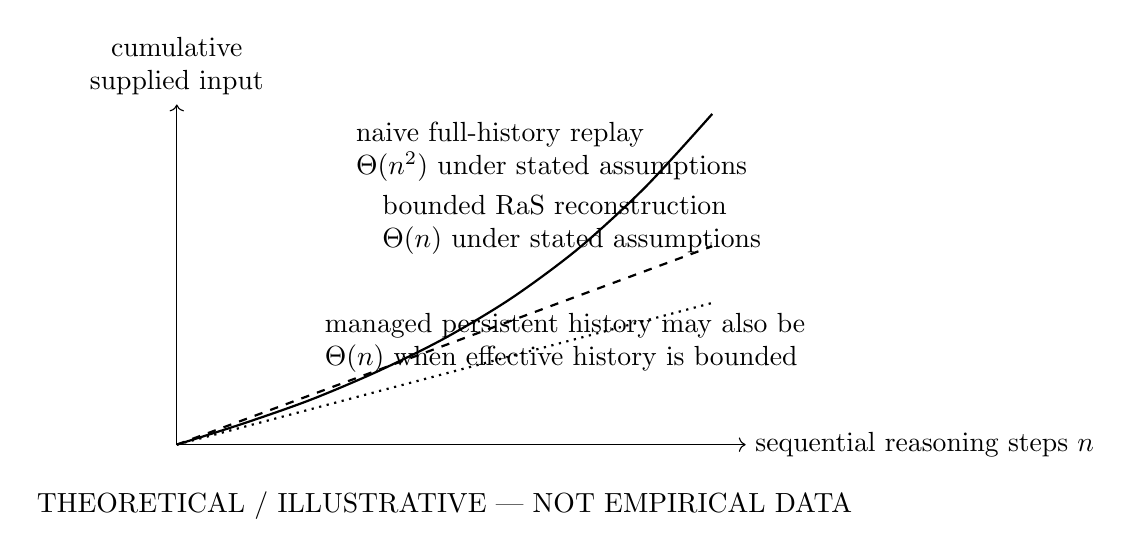
\begin{tikzpicture}[x=0.85cm,y=0.6cm]
\draw[->] (0,0) -- (8.5,0) node[right]{sequential reasoning steps $n$};
\draw[->] (0,0) -- (0,7.2) node[above,align=center]{cumulative\\supplied input};
\draw[thick] plot[smooth] coordinates {(0,0) (1,0.45) (2,0.95) (3,1.55) (4,2.25) (5,3.1) (6,4.15) (7,5.45) (8,7)};
\draw[thick,dashed] (0,0) -- (8,4.2);
\draw[thick,dotted] (0,0) -- (8,3.0);
\node[align=left] at (5.6,6.2) {naive full-history replay\\$\Theta(n^2)$ under stated assumptions};
\node[align=left] at (5.9,4.65) {bounded RaS reconstruction\\$\Theta(n)$ under stated assumptions};
\node[align=left] at (5.8,2.15) {managed persistent history may also be\\$\Theta(n)$ when effective history is bounded};
\node[below,align=center] at (4,-0.8) {THEORETICAL / ILLUSTRATIVE --- NOT EMPIRICAL DATA};
\end{tikzpicture}

\caption{THEORETICAL / ILLUSTRATIVE --- NOT EMPIRICAL DATA. Quadratic growth is the naive full-history replay stress case; bounded reconstruction is a conditional RaS stress case. Persistent agents with bounded effective history can also have linear cumulative supplied input.}
\label{fig:context-growth}
\end{figure}

\subsection{Rediscovery is allowed to defeat RaS}

Handoff Debt provides direct evidence that repository-only successor agents can pay substantial rediscovery cost after interrupted tasks \citep{kc2026handoff}. RaS does not explain this away: if the same effect remains large after \emph{accepted} transition boundaries, it weakens the practical thesis.

Future experiments should capture:
\begin{itemize}
    \item reconstruction-attributed input tokens;
    \item repository bytes and number of files inspected;
    \item repository, symbol, dependency, and history searches;
    \item model and tool calls;
    \item reconstruction elapsed time and total task elapsed time;
    \item observable cache hits/misses or cached/uncached tokens;
    \item retries and escalations attributable to missing or incorrect reconstruction.
\end{itemize}

The proposed Reconstruction Token Fraction remains descriptive:
\begin{equation}
\mathrm{RTF}=
\frac{T_{\mathrm{reconstruction,input}}}
{T_{\mathrm{RaS,total~input}}}.
\label{eq:rtf}
\end{equation}
RTF alone cannot establish efficiency: a low fraction can coexist with high total cost, and a high fraction can be acceptable if total outcome-normalised resource use is low. Report the numerator and denominator as well as the ratio.

\subsection{Do not double-count conceptual cost components}

The original additive equations risked treating reasoning, context, and agent-state cost as mutually exclusive even though provider billing and inference work can overlap those concepts. The audit replaces them with a measured resource vector:
\begin{equation}
\mathbf{Z}_c=
(T_{\mathrm{in}},T_{\mathrm{out}},N_{\mathrm{model}},N_{\mathrm{tool}},
B_{\mathrm{repo-read}},N_{\mathrm{files}},t_{\mathrm{recon}},t_{\mathrm{total}},
N_{\mathrm{retry}},C_{\mathrm{billed}})
\label{eq:resource-vector}
\end{equation}
for condition $c$, with elements reported only where observable and with $C_{\mathrm{billed}}$ included only when exposed by the provider or metered service.

\begin{table}[htbp]
\centering
\small
\caption{Audit classification of economic/resource quantities. “Observable” means available to the experiment, not necessarily a direct measure of provider-internal cost.}
\label{tab:cost-observability}
\begin{tabularx}{\textwidth}{@{}lX X@{}}
\toprule
Class & Examples & Permitted use \\
\midrule
OBSERVABLE & Input/output tokens exposed by API, model/tool calls, repository bytes/files read, searches, elapsed time, retries, provider-billed charge when exposed & Report directly; compare outcome-normalised values across conditions \\
PARTIALLY OBSERVABLE & Cached-token counters, prompt-cache hits, session persistence indicators, opaque provider usage categories & Report with interface/version and limitations; do not infer hidden implementation \\
UNOBSERVABLE & Exact GPU allocation, KV-cache residency cost, internal storage/scheduling amortisation, provider margin & Do not label as measured saving; discuss only as theoretical implication \\
\bottomrule
\end{tabularx}
\end{table}


A monetary comparison may sum \emph{mutually exclusive metered charges} actually observed by the experiment. It must not add speculative “reasoning cost”, “KV-cache cost”, “GPU cost”, and subscription price as if those were independent measured quantities.

Three categories remain:
\begin{itemize}
    \item \textbf{OBSERVABLE}: experiment-side tokens/calls/reads/times and provider-billed usage when exposed;
    \item \textbf{PARTIALLY OBSERVABLE}: cache behaviour, retained session state, or provider-reported categories whose implementation is not transparent;
    \item \textbf{UNOBSERVABLE}: internal GPU scheduling, exact KV-cache residency cost, storage amortisation, hidden cache implementation, and provider margin.
\end{itemize}

LLM-serving research shows that KV-cache management and prefill/decode scheduling affect throughput \citep{kwon2023vllm,zhong2024distserve,qin2024mooncake}. It does \emph{not} justify inferring that closing a conversation releases a dedicated GPU allocation or that RaS yields a particular infrastructure saving. Infrastructure effects remain conditional implications requiring separate serving experiments.

\section{Tiered Execution}
\label{sec:tiered}

Tiered execution is \textbf{not logically necessary for RaS}. It is a secondary architecture that becomes convenient when reasoning persistence, execution state, and operational privilege are separated. The core continuity experiment must therefore be able to compare persistent-history and forced-reset conditions without changing executor quality.

A high-capability reasoner may be useful for architecture, decomposition, difficult causal reasoning, complex debugging, review, trade-off analysis, evidence interpretation, and work-package creation. A separate worker may perform repository edits, compilation, test execution, formatting, linting, Git operations, and tightly constrained environment interaction.

\begin{table}[htbp]
\centering
\small
\caption{Illustrative capability separation for tiered execution.}
\label{tab:reasoner-executor}
\begin{tabularx}{\textwidth}{@{}lX X@{}}
\toprule
Function & High-capability reasoner & Execution worker \\
\midrule
Architecture/decomposition & Primary & Follow bounded plan \\
Complex causal debugging & Primary & Collect evidence / execute checks \\
Repository editing & May propose patch & Primary operational role \\
Compiler/tests/lint & Interpret difficult evidence & Execute repeatedly \\
Git operations & Usually propose/approve & Restricted implementation actions \\
Environment access & Minimal where possible & Scoped to required tools \\
Production credentials & Not implied & Not implied \\
\bottomrule
\end{tabularx}
\end{table}


Let $N_R$ and $N_E$ denote reasoning and execution operations and let $c_R$, $c_E$, and $C_O$ denote their accounting-unit costs and orchestration overhead. Under the deliberately simplified accounting model:
\begin{align}
C_M&=(N_R+N_E)c_R,\
C_T&=N_Rc_R+N_Ec_E+C_O.
\end{align}
Therefore $C_T<C_M$ exactly when:
\begin{equation}
N_E(c_R-c_E)>C_O.
\label{eq:tiered}
\end{equation}

This inequality is elementary accounting, not a research contribution. It is retained only to expose the condition that hand-off overhead and quality failures must be included before declaring tiering cheaper. The quantities are not assumed to be monetary, mutually constant, or directly observable across providers.

Recent work independently studies modular repository exploration with lower-cost models and finds useful quality/cost operating points for issue localisation \citep{awad2026exploration}. Model routing is also established prior work \citep{ong2024routellm}. RaS therefore claims no novelty for using cheaper models for suboperations.

Tiered execution can fail because a work package omits a constraint, the executor cannot handle an unexpected state, tool permissions differ, or repeated hand-offs cause retries and re-entry. Any economic study must count those failures.

\paragraph{P0 scope.}
Condition D is removed from the primary P0 causal comparison. P0 should first establish whether conditions A and B can be matched except for predecessor reasoning-session history. A small preregistered semantic-state ablation may be exploratory. Tiered execution belongs in a later experiment once the continuity intervention itself is identifiable.

\section{Tests as an Executable Semantic-State Carrier}
\label{sec:executable-memory}

Tests can preserve executable behavioural constraints produced by earlier engineering work. That observation is ordinary software engineering, not a RaS novelty claim. The RaS-specific question is whether such durable constraints reduce the marginal value of predecessor reasoning-session history after an accepted transition.

Suppose an engineering episode establishes:
\begin{quote}
Duplicate requests must not create duplicate effects.
\end{quote}
A repository may preserve this through an idempotency test. A future actor can then detect a violating implementation without receiving the conversation that originally discovered the invariant.

Tests have useful continuity properties:
\begin{itemize}
    \item executable behavioural knowledge;
    \item versioning alongside constrained code;
    \item model-independent evaluation;
    \item CI integration;
    \item regression detection;
    \item human reviewability.
\end{itemize}

But tests are not a complete memory system. They may omit architectural rationale, rejected alternatives, business intention, security intent, operational assumptions, and behaviours not exercised by the suite. An implementation can also overfit visible tests.

Accordingly, this paper avoids the stronger slogan “tests are memory”. Tests are one class of durable semantic-state carrier among source, schemas, architecture records, build rules, history, and documentation. Their marginal contribution is an empirical ablation question.

Context-file research provides a cautionary analogue. Repository-level AGENTS.md-style files can increase exploration and cost without improving task success, and controlled studies report small or null correctness effects depending on agent/task composition \citep{gloaguen2026agentsmd,khatri2026contextfiles}. More durable context is therefore not automatically better context.

The experiment must also avoid circularity. Visible tests can communicate constraints, so they cannot be the only acceptance oracle. Hidden behavioural verification should be stored outside the experimental workspace and should accept equivalent correct implementations rather than compare against the historical patch text.

\section{Durable Documentation and Selective Retention}
\label{sec:durable-docs}

Code and tests do not necessarily preserve why an architectural boundary exists, why an alternative was rejected, what security assumption is active, or which migration phase remains incomplete. Some information may therefore require explicit durable semantic representation.

RaS does not advocate dumping complete reasoning transcripts into Markdown. Guo's Git-bound memory work shows one legitimate alternative architecture in which session-derived episodes and decisions are deliberately persisted and retrieved \citep{guo2026gitmemory}. RaS tests whether some accepted boundaries can avoid needing that predecessor-session memory; it does not claim transcript persistence is inherently wrong.

A conceptual retention heuristic is:
\begin{equation}
P_{\mathrm{reuse}}(x)L_{\mathrm{missing}}(x)
>
C_{\mathrm{persist+retrieve}}(x),
\label{eq:retention}
\end{equation}
where the terms represent reuse likelihood, loss if missing, and preservation/retrieval cost. The expression is not an estimable production formula and is not used as an experimental statistic.

Candidate durable documentation includes architecture decisions, operational constraints, security boundaries, migration state, non-obvious business intent, and rejected alternatives whose repetition would create meaningful risk.

But more context can hurt. Gloaguen et al. report that repository-level AGENTS.md context files can reduce success while increasing inference cost \citep{gloaguen2026agentsmd}; Khatri reports bounded null correctness effects in a controlled two-agent ablation \citep{khatri2026contextfiles}. These results make documentation quality and selectivity empirical variables rather than presumed advantages.

Condition C should therefore ask:
\begin{quote}
\textbf{Which durable repository artefacts have marginal continuity value at accepted task boundaries?}
\end{quote}
It should not ask whether agents fail after deleting large amounts of useful state.

A successful RaS architecture may ultimately require selective semantic documentation. If the amount of specially curated state required grows comparably to the predecessor history it replaces, or only works when tailored by an author who already knows the future tasks, that is evidence against the strong state-economics/generalisation claim.

\section{Security and Least Privilege}
\label{sec:security}

RaS does not establish a security property. It \emph{permits} an architecture in which reasoning lifetime, execution privilege, and credential lifetime are independently scoped. That distinction is important.

A high-capability reasoner may need repository read access and permission to propose a patch or bounded work package. An executor may need workspace write access, compiler/test access, restricted Git, and tightly scoped environment actions. Production credentials may belong to neither. If policy is enforced outside the model, such separation can reduce the permissions held by any single component.

This is a \textbf{RaS-enabled architecture}, not proven security improvement. Prompt instructions are not access control; repository permissions, sandboxes, network policy, credential brokers, command allowlists, approval gates, and independently collected validation must enforce boundaries.

Threats include:

\paragraph{Prompt injection and poisoned semantic state.}
Malicious comments, instruction files, generated documentation, issue text, commit metadata, and other repository artefacts can manipulate reconstruction. Durable generated state can propagate an attack to future fresh reasoners.

\paragraph{Malicious tests and verifier-shaped behaviour.}
Tests are executable inputs to agent decisions and can themselves be compromised. Visible test success cannot be assumed to imply safe behaviour.

\paragraph{Compromised dependencies.}
Build systems may execute dependency hooks or scripts. Canonicalisation of the workspace does not make external dependencies trustworthy.

\paragraph{Work-package or patch injection.}
A compromised reasoner can craft a proposal intended to exploit the executor; a compromised executor can alter the requested patch, falsify local evidence, or attempt privilege escalation.

\paragraph{Secrets in authoritative state.}
A repository can accidentally contain credentials or sensitive data. Making repository state central to reconstruction increases the importance of provenance, secret scanning, and access controls; RaS does not make such content safe.

\paragraph{Human approval boundaries.}
High-consequence operations may require explicit human approval even when reasoner, executor, and local tests agree.

Potential benefits such as reduced blast radius, narrower credential distribution, and shorter-lived capabilities remain \textbf{IMPLICATIONS}. They require adversarial evaluation before any security claim can be upgraded.

\section{Repository Resumability and State Reconstruction}
\label{sec:resumability}

Neither the Repository Resumability Index (RRI) nor the structured reconstruction-probe score is part of the accepted P1, P2 or Subject-C outcome set. This section specifies descriptive and future instrumentation for a separate falsification route: a fresh reasoner may preserve behavioural success yet incur enough rediscovery cost or reconstruction error to make disposal unattractive. No RRI or reconstruction-probe score is reported as an executed empirical result in this paper.

Forced reset creates at least two separable questions:

\begin{enumerate}
    \item Did the fresh reasoner reconstruct the task-relevant accepted project state accurately?
    \item Did the resulting engineering transition satisfy the behavioural verifier?
\end{enumerate}

A binary task outcome alone cannot distinguish those mechanisms.

\subsection{Repository Resumability Index}

RRI is retained as a \emph{descriptive project metric}:
\begin{equation}
\mathrm{RRI}
=
\frac{\text{successful verified continuations after eligible forced resets}}
{\text{eligible forced resets}}.
\label{eq:rri}
\end{equation}

It is not a novel estimator of causality and it is not a substitute for the matched A/B comparison in Section~\ref{sec:sufficiency}. Easy tasks can inflate an aggregate RRI, tasks need not be equally difficult, and RRI mixes reconstruction and implementation capability.

An eligible reset is one for which:
\begin{itemize}
    \item the canonical allowed starting state was materialised correctly;
    \item the reset and contamination gates passed before model invocation;
    \item the current task and stable experimental instructions were available;
    \item the declared model/configuration and tool environment were available;
    \item no preregistered infrastructure-failure condition occurred before the agent could be tested.
\end{itemize}

A successful continuation requires the preregistered behavioural verifier to pass; compilation, textual similarity, agent self-report, or resemblance to the historical patch are insufficient.

In a future study that executes this metric, report RRI by task/depth and repository, with uncertainty intervals only when the number and dependence structure of repeated observations justify them. In addition, report \emph{complete-sequence success}: whether an entire dependent task chain reaches every accepted state without an agent failure. This prevents strong performance on early/easy tasks from hiding continuity collapse later in the programme.

\subsection{State-reconstruction probe}

A future reconstruction-cost study can require the fresh reasoner, before editing in reset conditions, to produce a structured report containing only inspectable state:
\begin{itemize}
    \item relevant architecture and components;
    \item current externally observable behaviour;
    \item constraints and invariants;
    \item relevant tests and evidence paths;
    \item prior accepted work that matters to the current task;
    \item work still required;
    \item uncertainty and known unknowns.
\end{itemize}

The probe must not request hidden chain-of-thought and must be stored outside the subject workspace. It must never be injected into later tasks.

A preregistered scoring rubric should derive objective items from hidden task ground truth: required components identified, constraints recovered, relevant verifier-facing behaviour described, and critical false claims or omissions. Where human scoring is unavoidable, evaluators should be blinded to condition when feasible and agreement should be reported.

The probe separates:
\begin{equation}
R_t \rightarrow \widehat{S}_t
\end{equation}
from:
\begin{equation}
\widehat{S}_t \rightarrow \text{verified engineering transition},
\end{equation}
where $\widehat{S}_t$ is the reportable estimated task-relevant state. It does not claim to recover private reasoning state.

\section{Forced-State-Reset Evaluation and Experimental Method}
\label{sec:method}

The central intervention removes predecessor reasoning-session continuity after an \emph{accepted} engineering transition and tests whether a fresh reasoner can continue a dependent programme from the same authoritative project state.

P0 was the original methodology pilot. It was executed exactly once and classified \mixedstatus; its A/B correctness outcome is not treated as causally interpretable and the pilot is not rerun. The P0 protocol remains historical method context. P1 and P2 are methodology-corrected Subject-B studies, and Subject C is one independent cross-repository replication step. Their results are reported separately and are not pooled.

The task-solving model is stochastic. The same repository state, task, prompt, model and execution configuration can produce different candidate code and verifier outcomes on another run. Repetitions therefore sample stochastic condition behaviour; matched agreement is not deterministic equality. Subject C has only three repetitions per task and nine matched task-by-repetition units. Its 30 behaviour observations are nested within those units and task contracts and must not be analysed as 30 independent experimental replicates. No equivalence, non-inferiority or superiority margin/test was introduced after observing the data.

\subsection{Study scope and public-safe task characterisation}

The private subject identities and historical source boundaries are withheld under the declared evidence boundary, but the selection and execution shape is frozen publicly. Subject C was selected from 22 candidate repositories: five met the preregistered eligibility rules and 17 were excluded. The deterministic selection procedure then chose three eligible sequential, locally testable historical task chains. Each selected task was executed three times per condition, producing 18 scheduled/model-active runs and nine matched task-by-repetition units. The task-solving runtime was frozen before execution, including the model, CLI/runtime, sandbox policy, condition mapping procedure and future-history controls. These counts describe the study population actually sampled; they do not imply that the three tasks or one additional repository represent software engineering generally.

P1 used three matched sequential tasks. P2 used four tasks, three repetitions and two conditions, producing 24 executions and 12 matched task-by-repetition pairs. Subject C deliberately changed repository/subject rather than pooling evidence with Subject B. The public records describe task counts, behavioural contracts, selection rules and execution controls while withholding private source material that would reveal the subject or hidden verifier implementation.

\subsection{Causal target}

The primary comparison is:

\paragraph{A --- Persistent-history control.}
The high-capability reasoner retains the predecessor reasoning-session history defined by the experimental chain while receiving the frozen task-specific authoritative state.

\paragraph{B --- Forced reset.}
A fresh high-capability reasoning session receives no predecessor conversation, hidden summary, copied reconstruction or resume state while receiving the same frozen task-specific authoritative state.

The intended treatment is \textbf{availability of predecessor reasoning-session history}. Everything else capable of materially affecting outcome must be matched, isolated or explicitly treated as a limitation.

The experiments do not compare “repository” against “no repository”, nor do they require generated code from one experimental task to become the next task's state. Each task receives its preregistered historical PRE boundary so A/B repository state remains matched; in persistent chains only the defined reasoning/session continuity carries forward.

\subsection{Canonical task-boundary materialisation}

Before every experimental task in both conditions, the harness must materialise the same accepted task boundary into a clean workspace. Persistent A must not inherit untracked files or tool residue merely because its reasoning session persists.

Relevant invariants include:
\begin{itemize}
    \item allowed repository/source state at the boundary;
    \item tracked and untracked workspace contents;
    \item system/developer experiment instructions and current task text;
    \item model identifier/runtime and exposed configuration;
    \item tool schema, executor implementation and privilege boundary;
    \item language/toolchain and environment policy;
    \item network policy;
    \item correctness oracle and acceptance rule.
\end{itemize}

Shell history, editor state, temporary files, previous-agent scratch files, local databases and generated summaries must not become hidden condition-specific continuity channels.

\subsection{Prompt, model and hidden-state controls}

The task contract and stable experiment instructions must be frozen before execution. Condition differences may expose predecessor session history only according to the preregistered treatment. Account-level or provider-side memory that cannot be controlled is a threat to identifiability and must be disclosed if present.

Prompt/context caching is not itself the behavioural treatment. Exposed cache counters may be reported for resource accounting, but behavioural conclusions must not be inferred from unobservable provider internals.

\subsection{Future-history and task-leakage controls}

Historical task workspaces must exclude post-cutoff solution information. A fail-closed future-history/leakage gate must prevent access to future repository objects, refs, alternate object stores, source-repository links, hidden patches, task-generation material or other post-cutoff solution artefacts.

Information legitimately present in the accepted PRE state is allowed even when it is useful. Leakage is information from the future or from hidden task/verifier construction that the task-solving agent was not meant to receive.

\subsection{Behavioural verification}

Correctness evidence must be frozen before outcome inspection and must test disclosed task requirements without requiring the historical textual implementation. Hidden verifier implementations may remain private, but the behavioural requirements they enforce may not be secret requirements.

The Subject-C verifier package was independently qualified before experimental output adjudication. Across its three selected historical tasks, all three PRE states produced the expected failing result and all three POST states produced the expected passing result. Ten targeted negative controls were all detected; ten alternate-valid implementations were all accepted; and ten adversarial false-positive controls were all rejected. The implementation-independence check and all three future-history gates passed. Project build/compiler/public-test/lint results were not used as Subject-C correctness evidence. An earlier verifier version that was too coupled to the historical implementation was rejected rather than used.

\subsection{Development and infrastructure are outside the experiment}

Harness development, authentication, ACL/materialisation work, launcher/controller debugging, CLI compatibility work, staging/transport problems, environment repair and disposable pre-experiment smoke runs are \textbf{engineering provenance, not experimental outcomes}.

A Subject-C experimental unit began only when its valid locked task-solving model execution became genuinely model-active. Once model-active, the unit was consumed and could not be rerun for quality. Pure transport or infrastructure failure before task-model activity did not create a behavioural observation. If continuing would have required changing a frozen experimental invariant after model activity, the experiment would have stopped rather than silently repairing or rerunning the unit.

This boundary prevents infrastructure work from appearing as experimental failures, retries, denominators, condition outcomes or correctness observations. Historical P1/P2 records may retain process-event provenance, but such metadata is not part of their behavioural correctness denominator unless the relevant protocol explicitly defines it as an experimental model-active observation.

\subsection{No human rescue and outcome selection}

After a valid task-model run becomes active, prohibit hints, file pointers, copied information, prompt adjustment, manual candidate edits, cross-condition rescue and selective quality reruns. Repetitions are experimental repetitions, not retries. Best-of-$N$ outcome selection is prohibited unless preregistered as a different experiment.

Subject C executed all 18 scheduled model-active units exactly once, froze all outputs before correctness adjudication, and then blind-adjudicated the frozen candidates before unsealing the condition mapping.

\subsection{Interpretation discipline}

P0 is methodology/falsification history, not causal A/B correctness evidence. P1 observed equal non-zero sample performance. P2 observed equal floor-level sample performance and therefore does not positively demonstrate successful behavioural preservation. Subject C observed mostly matching behaviour outcomes plus five discordances in a small stochastic sample. None of these designs establishes superiority, equivalence, non-inferiority or a population-level effect.

Confirmatory future work would require a declared task population, more independent repetitions/repositories, dependence-aware statistical analysis, preregistered stopping/missing-data rules and a scientifically justified margin if equivalence or non-inferiority is claimed.

\subsection{Outcome and resource telemetry}

Behavioural reporting uses frozen verifier-defined outcomes, task-level results and matched condition comparisons. Resource/reconstruction telemetry is a separate claim family and was not part of the accepted P1, P2 or Subject-C behavioural outcome set. The Repository Resumability Index and structured reconstruction probe in Section~\ref{sec:resumability} therefore specify descriptive or future instrumentation; no RRI or reconstruction-probe score is presented as an executed result in this paper. Where observable, future studies should report input/output tokens, model/tool calls, repository reads/searches, elapsed time, retries, cache counters and provider-billed usage. Provider-internal GPU scheduling, exact KV-cache cost, storage amortisation and margin are not inferred from client telemetry.

\section{AI Assistance and Author Responsibility}
\label{sec:ai-assistance}

Generative AI systems were used as research-engineering and authoring tools during this project. Their uses included repository analysis, implementation and test support, experiment-harness and documentation work, adversarial review assistance, and manuscript drafting and editing. Where AI systems were themselves part of the experimental treatment or execution environment, their role and controls are described in the experimental method and retained evidence records.

The human author defined the research questions, experimental boundaries, acceptance criteria, preregistration and no-rerun rules, adjudication requirements, claim limits, and publication decisions; reviewed and accepted or rejected AI-assisted outputs; and remains solely responsible for the integrity of the evidence, citations, interpretation, and final manuscript. AI systems are not authors and no authorship or scientific accountability is attributed to them.

\section{Results}
\label{sec:results}

P0 was executed exactly once and classified \mixedstatus; its A/B correctness outcome is not treated as causally interpretable and P0 is not rerun. The controlled evidence that follows consists of bounded Subject-B P1/P2 samples and one independent Subject-C cross-repository replication step. None is a general validation of Repository-as-State.

\subsection{Subject-B P1}

P1 compared persistent-session and fresh-session conditions across three matched tasks. Condition A and Condition B each satisfied 18/30 governing behaviours. The matched vectors had 30 agreements and 0 disagreements; both conditions passed two of the three tasks. This is bounded positive evidence for the narrow observation that the two conditions produced the same verifier-defined behaviour vector in this P1 sample. Because the task-solving model is stochastic and the sample is small, it is not deterministic equality, formal equivalence, non-inferiority, universal sufficiency, or a resource-cost result.

\subsection{Subject-B P2}

P2 used four tasks, three repetitions, two conditions, 24 executions and 12 matched task-by-repetition pairs. The four task contracts define 13 governing behaviours per repetition, giving 39 behaviour observations per condition. Both conditions satisfied 0/39 and failed 39/39. The matched vectors had 39 agreements and 0 disagreements, and candidate-level overall verifier passes were 0/12 in both conditions.

The P2 result is a floor effect. No behavioural correctness difference was observed between the persistent-session and fresh-session conditions in this P2 sample, but because both conditions were at the floor, P2 does not demonstrate successful behavioural preservation by either condition and cannot be interpreted as evidence of behavioural equivalence or repository-state sufficiency. Its value is therefore methodological and falsificatory rather than positive preservation evidence. P1 and P2 are not pooled.

\subsection{Subject-C cross-repository replication step}

Subject C used three sequential tasks, three repetitions per condition, 18 scheduled/model-active units and nine matched task-by-repetition units. Persistent-session Condition A satisfied 12/30 governing behaviours; fresh-session Condition B satisfied 15/30. Candidate full passes were tied at 2/9 per condition. Of 30 matched behaviour observations, 25 agreed and five disagreed; one disagreement favoured A and four favoured B.

The task-level pattern is essential. SC\_T01 was A 1/9 and B 5/9, with five agreements and four disagreements. SC\_T02 was 0/9 in both conditions, with nine agreements and no disagreements. SC\_T03 was A 11/12 and B 10/12, with 11 agreements and one disagreement. The aggregate therefore must not be presented as a general fresh-session win.

The 30 behaviour observations are not 30 independent experimental replicates. They are nested within nine matched task-by-repetition units, and multiple behaviours are scored from the same candidate/task output. In Condition A, the three task outputs within a repetition also share one persistent reasoning-session chain. The current analysis is descriptive and does not treat nested behaviour rows as independent Bernoulli trials.

The task-solving model is stochastic: repeating the same state, task, prompt, model and configuration can produce different candidates and verifier outcomes. With only three repetitions per task, the four-to-one discordant direction is descriptive only and may reflect ordinary run-to-run variation rather than a systematic condition effect. Subject C does not establish superiority, inferiority, equivalence or non-inferiority.

Subject C is an independent cross-repository replication step toward broader external validation. One additional subject/repository does not by itself satisfy the programme roadmap's eventual target of multiple unrelated repositories, task classes, languages/architectures and broader variation. Some public artefact filenames retain `level3` because that was the internal programme stage name; the label is not a claim of population-level external validity.

P1, P2 and Subject C are reported separately and are not numerically pooled.

\subsection{Adjudication integrity and resource boundary}

P2's first adjudication attempt remains preserved as invalid history: placeholder calls produced zero valid adjudications, premature unblinding occurred, and a later sealed-verifier diagnostic result was excluded. The accepted recovery used fresh blinded adjudications, froze them before unblinding, and repaired only a derived denominator error; no P2 task-model reruns were added.

Subject C froze all 18 model-active outputs before blind semantic adjudication. No project build, compiler/typechecker, project/public test, or lint result was used as its correctness oracle. Infrastructure/harness events are engineering provenance and are excluded from experimental failure counts, retries, denominators and condition outcomes.

Resource/reconstruction telemetry remains separate and descriptive. The current controlled evidence does not establish a cost, speed, token, monetary, security or provider-serving advantage. No RRI or structured reconstruction-probe score forms part of the accepted P1, P2 or Subject-C result set.

The project uses the claim categories in Table~\ref{tab:claim-categories} to prevent theoretical, observed, and hypothetical statements from being silently presented as findings.

\begin{table}[htbp]
\centering
\small
\caption{Claim/evidence categories used throughout the project.}
\label{tab:claim-categories}
\begin{tabularx}{\textwidth}{@{}lX@{}}
\toprule
Category & Meaning \\
\midrule
THEORETICAL & Follows from stated mathematical or architectural assumptions \\
OBSERVED & Motivating practical observation, not a controlled experiment \\
EMPIRICAL & Supported by controlled measured evidence under a versioned protocol \\
EXTERNAL & Supported by cited third-party or first-party external evidence \\
HYPOTHESIS & Testable proposition not yet established by the project \\
IMPLICATION & Conditional consequence if underlying premises are supported \\
\bottomrule
\end{tabularx}
\end{table}


\section{Reproducibility and Public Evidence Boundary}
\label{sec:reproducibility}

The Repository-as-State release distinguishes \emph{public auditability} from \emph{full independent reproduction}. The public repository contains the manuscript, protocol descriptions, public-safe result records, preregistration/lock summaries, output-freeze summaries, adjudication summaries, and cryptographic commitments needed to audit the published claim chain. It does not contain private subject source, private historical boundaries, private schedules or seeds, blind mappings, credentials, or hidden verifier implementation where disclosure would violate the experimental or confidentiality boundary.

The canonical public evidence chain is:
\begin{itemize}
    \item P0: preregistration/runtime records, raw result and post-experiment review, ending in \mixedstatus with no causal A/B correctness interpretation;
    \item Subject-B P1: public result record plus its preregistration, execution-lock, blinded-freeze, adjudication and interpretation commitments;
    \item Subject-B P2: preregistration binding, execution lock, output freeze, blind-adjudication recovery record, accepted result and public evidence summary;
    \item Subject C: selection/design, verifier qualification, V4 preregistration and execution lock, 18-run output freeze, blind adjudication and bounded cross-repository evidence summary.
\end{itemize}

The top-level \breakcode{REPRODUCIBILITY.md} and machine-readable \breakcode{results/public/repository-as-state-reproducibility-manifest-v1.json} enumerate the canonical files and accepted commitments for the v1.0 release.

For Subject C, the controlling public commitments include the V4 lock package SHA-256 \breakcode{9ffde0ba9974eab7efbba6d7ab644c3081fa534b211a7fa8f9aaf560d295ed13}, output-freeze package SHA-256 \breakcode{ff1616a03594f1afbdccf8d15bd841df74465eefd06d33fcb8a1de8af841a9e8}, semantic-verifier package SHA-256 \breakcode{18aa90e28afbf1f36d2aa909417cb436279ddf20fc8c99e516ae25f42f25c0cd}, blind-result commitment SHA-256 \breakcode{58e1cd7c375d847db5f7539f0afa636bc2b4643ebefcb3b53f055b3bc44fb64f}, and adjudication package SHA-256 \breakcode{0a0b23e6be9e30c042f908b84f3d5b684e9960820a4ec9115741298a0ac3b1ad}.

These commitments allow later comparison against retained private packages without publishing the hidden material itself. They do not allow an external investigator to recreate every private experimental byte solely from the public repository. The appropriate stronger test is independent replication on independently available subjects and verifiers, not disclosure-by-assertion.

\subsection*{Data and materials availability}

Public protocols, aggregate results, public-safe execution and adjudication records, reproducibility manifests, manuscript/source material and cryptographic commitments are available in the public Repository-as-State repository and its immutable v1.0 release. Private subject repositories, private historical boundaries, schedules or seeds that would reveal protected experimental material, blind mappings, credentials and hidden verifier implementations are withheld under the declared confidentiality and experimental boundary. The released package therefore supports audit of the published claim chain and limited reconstruction from public-safe artefacts; it does not claim byte-for-byte independent reproduction of private-subject executions.

The release also preserves the statistical unit boundary. Subject C contains nine matched task-by-repetition experimental units; its 30 matched behaviour observations are nested measurements and are not 30 independent replications. P1, P2 and Subject C are separate experiments and are not numerically pooled.

No new experiment, verifier execution, candidate repair, post-hoc statistical test, or reinterpretation was introduced during final release packaging. Venue-specific formatting, PDF generation, archival deposition and branch integration are publication operations outside the experimental programme and must not strengthen the accepted claims.

\section{Related Work and Narrowed Novelty Boundary}
\label{sec:related}

Hostile literature review materially narrows the novelty claim. Repository-backed agent memory, commit-history memory, sequential software evolution benchmarks, interrupted-task handoff evaluation, lower-cost repository exploration, durable execution, and repository-scale replaceable compute all predate this programme. RaS is defensible only if it credits those overlaps and focuses on the treatment they do not isolate.

\subsection{Repository-level agents and sequential software evolution}

SWE-bench and SWE-agent establish repository-level issue resolution and agent--computer interfaces \citep{jimenez2024swebench,yang2024sweagent}. OpenHands and its SDK provide sandboxed execution, lifecycle control, memory mechanisms, security features, and multi-model routing \citep{wang2024openhands,wang2025openhandsSDK}. SWE-STEPS already evaluates chains of dependent pull requests and shows that isolated-task evaluation can overstate long-horizon performance \citep{shastry2026swesteps}. RaS therefore cannot claim novelty for repository-level coding or sequential task chains.

Its narrower experimental variable is whether predecessor \emph{reasoning-session history} is needed after an accepted state transition when dependent task, model/runtime, tools and authoritative state are otherwise matched.

\subsection{The closest empirical challenge: interrupted-task handoff}

Handoff Debt is the closest direct empirical challenge identified in the reviewed literature \citep{kc2026handoff}. It freezes repository state at interruption points and compares successor agents receiving repository-only state, raw traces, summaries or structured notes. Context-bearing handoffs substantially reduce rediscovery effort relative to repository-only takeover in that setting, while solve-rate effects are smaller and model dependent.

That work defeats any broad claim that “the repository alone makes predecessor context unnecessary” or that repository-only reconstruction is automatically economical. The remaining distinction is the reset boundary: Handoff Debt interrupts partially completed tasks, while RaS studies accepted engineering boundaries. The current RaS correctness samples do not establish that the accepted-boundary distinction removes rediscovery cost; resource/economic evidence remains incomplete.

\subsection{Git-bound and repository memory}

Guo explicitly argues that agentic-development memory should be Git-bound, linking assistant sessions to commit state and routing queries over structural maps, episodes and decision synthesis \citep{guo2026gitmemory}. This strongly overlaps the broad “repository as memory” intuition, but persists session-derived information inside the memory system. RaS instead tests a condition in which predecessor reasoning-session state is absent after an accepted transition.

Other work uses commit history as non-parametric repository memory for code localisation \citep{wang2025repomemory} or builds online repository memory from historical commits to learn project-specific change patterns \citep{li2026learningcommit}. These results make clear that repository history can be useful memory while also warning that a current source snapshot may omit project-specific patterns.

\subsection{Repository context files}

Repository instruction files are established context mechanisms. Sun et al. document public Cursor rule files containing project context and engineering guidance \citep{sun2026cursorrules}. Gloaguen et al. find that AGENTS.md-style context files can reduce task success and raise inference cost despite increasing exploration \citep{gloaguen2026agentsmd}. Khatri's ablation reports bounded/null correctness effects in its studied setting \citep{khatri2026contextfiles}. These findings weaken any assumption that more curated repository documentation automatically improves resumability.

\subsection{Repository exploration, routing and agent memory}

Repository exploration is itself measurable and costly. Awad and Ivanov evaluate lower-cost explorer models and identify quality/cost operating points for localisation \citep{awad2026exploration}; RouteLLM studies learned model routing \citep{ong2024routellm}. MemGPT and later memory work establish managed external memory as a broad agent design space \citep{packer2023memgpt,du2026memory,luo2026memory}. Consequently, model routing, cheaper exploration and external memory are not RaS novelty claims.

\subsection{Durable execution and inference-state management}

Durable Functions formalises stateful workflows under compute--storage separation and replay \citep{burckhardt2021durable}; durable AI workflow research also studies semantic isolation across pauses and continuations \citep{mozafari2026semantic}. RaS does not claim to invent checkpoint/restart or transactional computation. Its object is semantic engineering continuity for a fresh nondeterministic reasoner.

PagedAttention/vLLM, DistServe and Mooncake show that KV-cache allocation and serving architecture are more complex than one conversation occupying one dedicated GPU \citep{kwon2023vllm,zhong2024distserve,qin2024mooncake}. RaS therefore makes no provider-internal saving claim from session disposal.

Cursor Continuity persists repository-serving state over replaceable compute \citep{marti2026continuity}. This is repository-infrastructure precedent, not an agent-continuity experiment.

\subsection{What remains plausibly distinct}

After removing broad claims, the reviewed work did not identify an exact prior matched experiment combining all of the following:

\begin{enumerate}
    \item dependent software-engineering tasks separated by accepted/validated boundaries;
    \item deliberate removal of predecessor high-capability reasoning-session state after those boundaries;
    \item a matched history-retaining control with task/model/tools/environment and accepted state otherwise controlled;
    \item correctness reporting that allows forced reset to lose; and
    \item explicit reconstruction/resource accounting as a separate possible falsifier.
\end{enumerate}

This is a provisional literature-search finding, not proof that no such prior work exists. The broad repository-memory and sequential-agent space is already crowded, and a newly discovered exact predecessor study would narrow the novelty further.

P1, P2 and Subject C now provide bounded empirical samples of the behavioural intervention, but they do not transform the novelty claim into a general theory. The economic/reconstruction part of the proposed distinction remains particularly under-tested because the current resource evidence is incomplete.

\section{Threats to Validity}
\label{sec:threats}

RaS is unusually vulnerable to validity failures because its treatment is information availability. A convincing study must control not only prompts but hidden state channels through which predecessor work can survive.

\subsection{Construct validity}

\textbf{Repository sufficiency is conditional, not intrinsic.} Success can depend on task class, depth, model, tool contract, environment and repository quality. The paper therefore reports matched behavioural observations rather than claiming latent action-distribution equality.

\textbf{RRI is descriptive.} It mixes reconstruction and implementation ability, can be inflated by easy tasks, and is not a causal estimator.

\textbf{Behaviour rows are not independent replications.} Multiple governing behaviours can be scored from one candidate/task output. In Subject C the 30 matched behaviour observations are nested within nine matched task-by-repetition units; the task outputs within each persistent-condition repetition also share one reasoning-session chain. Treating 30 behaviour rows as 30 independent trials would be pseudo-replication.

\textbf{Reconstruction accuracy and cost classifications require frozen rules.} Textual similarity can reward verbosity without understanding, and repository reading/search/model work needed to reconstruct lost context must not be silently moved outside the resource accounting.

\textbf{Economic observability is limited.} Client-visible tokens, calls and time do not reveal provider-internal GPU scheduling, KV-cache residency cost, storage amortisation or margin.

\subsection{Internal validity}

\textbf{Treatment confounding} remains the central risk. A new session can differ from a persistent one through prompts, provider account memory, prompt caches, tool sessions, executor state, shell history, untracked files, worktrees, environment variables, dependency caches or network state. The accepted studies use frozen task state and controlled execution boundaries, but provider/runtime specificity remains a limitation.

\textbf{Future-history leakage} is catastrophic. Historical workspaces must not expose future solution state through refs, packs, alternates, remotes, source links, generated artefacts or task-generation material. The accepted protocols use fail-closed isolation gates before task-model activity.

\textbf{Verifier leakage} invalidates behavioural testing if the task-solving agent can access hidden verifier implementation or undisclosed requirements. Subject C used an independently qualified implementation-independent semantic verifier whose implementation remained isolated from the experimental identity.

\textbf{Human rescue and outcome selection} can create an undeclared continuity channel. The accepted Subject-C run prohibited quality reruns, best-of-N selection, prompt changes and manual candidate repair after model activity.

\textbf{Infrastructure is not an outcome.} Authentication, ACL/materialisation, launcher/controller, transport/staging, CLI, Windows/environment and harness-development events are engineering provenance. They must not be counted as experimental failures, retries, observations, denominators or condition outcomes. The Subject-C experimental boundary began only when a valid locked scheduled task became model-active.

\textbf{Model stochasticity and provider drift} can produce outcome differences unrelated to state persistence. The same state, task, prompt, model and execution configuration can yield different candidate code and verifier outcomes. Subject C has only three repetitions per task, limiting precision and making its 4-to-1 discordant direction descriptive.

\subsection{Selection and author bias}

The programme uses a small number of subjects/repositories and remains author-led. P0/Subject-B are particularly exposed to author familiarity, historical survivor bias and repository discipline that may favour reconstruction. Subject C used a frozen discovery/selection protocol before outcome observation and was independent of Subject B, which mitigates but does not eliminate selection and investigator bias.

Historical tasks necessarily select work that reached a known accepted future state. Dead ends and ambiguous unsuccessful changes are underrepresented. Independent task construction and external replication remain necessary.

\subsection{External validity}

The programme now contains Subject-B and one independent Subject-C cross-repository replication step, but this is still a very small repository/task population and uses one model/runtime family. It does not establish generalisation across public repositories, languages, architectures, repository sizes, dependency widths, documentation/test quality, agent implementations or model families.

The roadmap's full Level-3 threshold calls for multiple unrelated repositories/task classes and broader structural variation. Subject C is one step toward that threshold, not completion of population-level external-validity evidence.

\subsection{Statistical conclusion validity}

The experiments are descriptive bounded samples. Small task/repetition counts cannot establish superiority, equivalence or non-inferiority. P1's complete matched agreement is not deterministic equality. P2 is at the correctness floor. Subject C has nine matched task-by-repetition units and only three repetitions per task; its five discordances are heterogeneous across tasks and do not support a stable condition-effect estimate.

No post-hoc significance, superiority, equivalence or non-inferiority test is added after observing Subject-C outcomes. Confirmatory inference would require a declared task population, more independent units, a dependence-aware analysis, missing-data/stopping rules, multiplicity handling where relevant, and a scientifically justified preregistered margin if equivalence/non-inferiority is the target.

P1, P2 and Subject C are separate experiments and must not be pooled into a single correctness statistic.

\subsection{Reproducibility boundary}

The public repository provides a coherent audit/commitment chain for the published design, locks, freezes and aggregate adjudication. It does not make private subject source, private historical boundaries, blind mapping or hidden verifier implementation public. Therefore the current record supports auditability and commitment checking, not full independent reproduction of every experimental byte from public material alone. Independent external replication requires independently available subjects/tasks/verifiers.

\subsection{Prior empirical evidence adverse to a strong thesis}

Handoff Debt reports substantial rediscovery overhead for repository-only successor agents on interrupted tasks \citep{kc2026handoff}. That intervention is not the same as post-acceptance RaS, but it is adverse prior evidence against any assumption that repository reconstruction is automatically efficient. The present correctness results do not resolve the economic question because reconstruction/resource evidence remains incomplete.

\subsection{Central falsification conditions}

RaS is weakened if fresh-session reset reduces verified task success in a properly powered preregistered study; complete-sequence success collapses with depth; reconstruction dominates resource use; persistent history consistently yields better outcomes; success depends on unusually tailored semantic documentation; or effects disappear across unrelated repositories/models. These remain future confirmatory questions rather than claims resolved by the current bounded samples.

\section{Discussion}
\label{sec:discussion}

The hostile audit changes how RaS should be interpreted. The broad intuition that “software repositories can act as memory” is not novel. Git-bound agent memory, commit-history memory, context files, repository maps, and sequential coding evaluation already exist \citep{guo2026gitmemory,wang2025repomemory,li2026learningcommit,shastry2026swesteps}. The potentially useful contribution is narrower: make \emph{accepted engineering boundaries} the disposal boundary and measure the value of predecessor reasoning-session history at those boundaries.

\subsection{The strongest adverse prior}

Handoff Debt shows that repository-only takeover of interrupted work can incur substantial rediscovery compared with context-bearing handoffs \citep{kc2026handoff}. RaS should not claim this evidence is irrelevant. It suggests that reasoning history can carry valuable information not yet represented in partial repository state.

The post-acceptance boundary remains the distinguishing hypothesis. The current P1/P2/Subject-C correctness samples do not settle the corresponding economic question because reconstruction/resource evidence is incomplete. A future valid resource study must therefore be allowed to find that behavioural continuation is possible while repository rediscovery is too expensive to justify session disposal.

\subsection{Decision-relevant semantic compression is ordinary engineering}

Software projects have always compressed design reasoning into code, tests, documentation, schemas, and history. Calling that “decision-relevant semantic compression” describes a useful mechanism but does not make it new. RaS concerns the possible \emph{architectural consequence}: because engineering externalises substantial decision-relevant state, persistent model history may have limited marginal value after some accepted boundaries.

That consequence must be measured, not inferred from the existence of tests or Git.

\subsection{Observed origin remains anecdotal}

The architecture was recognised through repeated practical use involving human orchestration, high-capability reasoning, local execution agents, deterministic evidence, and repository persistence. This remains motivation only. It is exposed to confirmation bias, task selection, author familiarity, survivor bias, model familiarity, human rescue, and undocumented assistance.

\subsection{Persistent agents may simply be better}

A negative outcome remains credible. Persistent history may save rediscovery, preserve rationale omitted from durable artefacts, and provide low-cost continuity when compaction and caching are effective. RaS may work only at coarse accepted boundaries, for local tasks, or in unusually disciplined repositories. Hybrid designs may dominate both permanent persistence and forced reset.

\subsection{What the accepted evidence says}

P1 found equal non-zero behavioural performance in its three matched tasks: 18/30 in each condition, 30 agreements and no disagreements. Because the model is stochastic and the sample is small, this is sample agreement, not proof of deterministic equality or equivalence.

P2 expanded the same-repository block to four tasks and three repetitions, but both conditions satisfied 0/39 behaviours, with 39 agreements, no disagreements and 0/12 candidate-level overall passes. Thus P2 detected no observed condition difference while providing no positive evidence that either condition successfully solved the Level-2 tasks. The floor effect prevents an equivalence interpretation.

Subject C adds one bounded cross-repository replication step. Persistent A satisfied 12/30 behaviours and fresh B 15/30; 25/30 matched behaviour observations agreed and five differed, with four disagreements favouring B and one A. Candidate full passes were tied at 2/9 per condition. Most discordance is in SC\_T01; SC\_T02 is at floor in both conditions; SC\_T03 is near ceiling and slightly favours A on behaviour count.

The 30 behaviour observations are nested within nine matched task-by-repetition units and are not independent experimental replicates. With only three repetitions per task and stochastic task solving, the 4-to-1 discordant direction is descriptive only and may reflect ordinary run-to-run variation. Subject C does not establish that fresh sessions are superior, persistent sessions inferior, or the conditions equivalent/non-inferior.

P1, P2 and Subject C are separate, unpooled samples. Taken together they demonstrate that post-acceptance reasoning-state persistence is experimentally testable and that outcomes can vary by task and study design; they do not establish a population-level condition effect.

\subsection{Cross-repository evidence is not full external validation}

Subject C is independent of Subject B and therefore improves the evidence beyond a single-repository programme. However, one additional subject does not satisfy the roadmap's full Level-3 threshold of multiple unrelated repositories/task classes, languages/architectures and broader structural variation. The appropriate description is a cross-repository replication step toward external validity, not generalisation.

\subsection{Human and AI complementarity is secondary}

Human and AI systems exhibit different capability profiles. Humans may contribute persistent goals, strategic problem selection, taste and risk judgement; AI systems may contribute synthesis, formalisation, critique and implementation leverage; deterministic systems provide executable checks. This describes the motivating workflow but is not part of the central causal claim.

\subsection{What a useful negative result would teach}

If reset fails because crucial rationale is absent, the study identifies a state-representation gap. If reset succeeds but reconstruction consumes most resources, the continuity hypothesis may survive while the economic hypothesis fails. If performance depends on tailored state files, RaS may reduce to a repository-documentation discipline rather than a general lifecycle property. If effects disappear on unrelated repositories or models, external validity is narrow.

The theory is useful only if those outcomes are allowed to count against it.

\section{Repository-State and Agent-State Scalability}
\label{sec:scalability}

The paper retains a distinction between repository-state scalability and agent-state scalability, but the latter now has an explicit definition.

\emph{Repository-state scalability} concerns storing, serving, and reconstructing repository objects and history as repository count and size grow. Cursor Continuity is a contemporary example of durable object/log state with replaceable repository-serving compute \citep{marti2026continuity}.

\emph{Agent-state scalability} is an architectural objective: the ability to increase the number or duration of concurrent long-horizon agentic programmes without proportionally increasing persistent \emph{high-capability reasoning-session state} requirements.

Figure~\ref{fig:scalability-stack} is conceptual.

\begin{figure}[htbp]
\centering
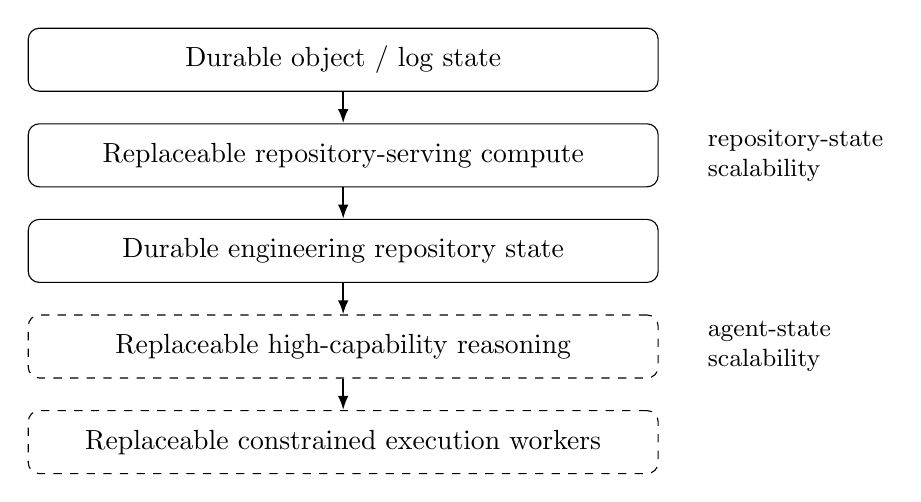
\begin{tikzpicture}[
node distance=4mm,
repo/.style={draw,rounded corners,align=center,minimum width=8cm,minimum height=8mm},
agent/.style={draw,dashed,rounded corners,align=center,minimum width=8cm,minimum height=8mm},
arrow/.style={-{Latex[length=1.8mm]},thick}
]
\node[repo] (object) {Durable object / log state};
\node[repo,below=of object] (serve) {Replaceable repository-serving compute};
\node[repo,below=of serve] (eng) {Durable engineering repository state};
\node[agent,below=of eng] (reason) {Replaceable high-capability reasoning};
\node[agent,below=of reason] (exec) {Replaceable constrained execution workers};
\draw[arrow] (object)--(serve);
\draw[arrow] (serve)--(eng);
\draw[arrow] (eng)--(reason);
\draw[arrow] (reason)--(exec);
\node[right=5mm of serve,align=left,font=\small] {repository-state\\scalability};
\node[right=5mm of reason,align=left,font=\small] {agent-state\\scalability};
\end{tikzpicture}

\caption{CONCEPTUAL --- NOT EMPIRICAL DATA. Repository-serving durability and high-capability reasoning-session persistence are distinct layers. Cursor Continuity supports only the upper repository-infrastructure precedent.}
\label{fig:scalability-stack}
\end{figure}

The two problems are independent. A scalable Git service does not imply that agents can resume without conversational history. Conversely, reasoning-session disposal does not require novel Git infrastructure.

Long-context inference creates serving-state and processing requirements, but production serving is more complex than one conversation occupying one dedicated GPU. PagedAttention manages KV-cache allocation \citep{kwon2023vllm}; DistServe separates prefill and decode resources \citep{zhong2024distserve}; Mooncake uses disaggregated KV-cache infrastructure \citep{qin2024mooncake}. Consequently, terminating a reasoning session does not map cleanly to a provider-internal resource saving.

The only defensible infrastructure statement at v0.1 is conditional: if a workload can reduce persistent high-capability reasoning-state requirements while preserving useful outcomes and without paying the same cost in reconstruction, a serving system \emph{may} have more scheduling flexibility or useful concurrency. This is an \textbf{IMPLICATION}, not a measured result.

A direct agent-state scalability claim therefore requires future workload-level serving experiments, not token accounting alone.

\section{Broader Authoritative-State Externalisation Principle}
\label{sec:authoritative-principle}

RaS may be a software-engineering-specific instance of a broader design question:

\begin{quote}
\textbf{Persist authoritative state. Reconstruct computation.}
\end{quote}

The hostile audit removes any suggestion that the paper has already formalised or established a general principle. Outside software engineering, the relevant state may live in CRM systems, transactional databases, ticket systems, event logs, document systems, infrastructure state, or combinations of those stores.

A future domain-specific experiment would need to ask behaviourally:
- what authoritative state is available at a valid recovery boundary;
- what predecessor model-native history is removed;
- which other state channels are matched;
- whether successor task outcomes degrade;
- how much reconstruction costs.

Software repositories are unusually favourable because they provide versioning, explicit diffs, executable tests, deterministic tools, schemas, reviewable text artefacts, and often reproducible builds. Other domains may rely more heavily on tacit, interpersonal, continuously changing, or externally governed information.

There is also no reason to assume one store is sufficient. A production engineering programme may require repository state plus deployment state, incident history, requirements, and tickets. Calling all of this “repository state” would obscure the causal treatment.

Accordingly, the Authoritative-State Externalisation Principle remains \textbf{FUTURE WORK / HYPOTHESIS}. RaS does not establish a general theory of intelligence or agent memory.

\section{Future Work}
\label{sec:future}

P0, P1, P2 and the bounded Subject-C cross-repository replication step are complete and must not be retrospectively rerun to obtain cleaner outcomes. Future work should extend the evidence population rather than modify accepted samples.

The highest-priority next scientific study is a larger preregistered distributional experiment with more independent repetitions, additional repositories and task families, and a dependence-aware statistical analysis fixed before outcomes. If equivalence or non-inferiority is a target, the margin must be justified in engineering terms and preregistered. The current P1/P2/Subject-C results cannot supply that margin post hoc.

The programme's full Level-3 external-validity threshold remains future work. One Subject-C cross-repository replication does not provide variation across multiple unrelated repositories, languages, architectures, repository sizes, dependency widths and documentation/test quality. Independent task selection and external replication would further reduce author/repository bias.

Reconstruction economics should be tested directly. A future study should measure reconstruction-attributed tokens, files/bytes read, searches, model/tool calls, elapsed time, retries and actual metered charges where exposed. It must count rediscovery as work and must not infer provider-internal GPU/KV-cache economics from client-side counters.

Semantic-state ablation should remove small preregistered information classes rather than broadly degrading the repository. The scientific question is which durable artefacts have marginal continuity value.

Tiered execution belongs in a separate experiment because changing executor capability would confound the core history treatment. Security claims likewise require adversarial evaluation rather than architectural argument alone.

Cross-model continuity remains particularly interesting. A design in which model family $M_A$ produces an accepted state and a different family $M_B$ resumes from it without predecessor model-native state would provide stronger evidence that continuity resides in external engineering state rather than a provider/model-specific session representation.

Reconstruction scaling should vary repository mass and dependency width while holding task semantics as constant as possible. Plain search, symbol indexes, static-analysis graphs, repository maps and model-guided retrieval can be compared without claiming any one is intrinsically RaS.

The broader Authoritative-State Externalisation Principle remains speculative. Software repositories have unusually strong versioning, diffability and verification properties; other domains may depend more heavily on tacit, continuously changing or externally governed information.

\section{Conclusion}
\label{sec:conclusion}

Hostile review narrows Repository-as-State rather than eliminating it.

The broad idea that Git or repositories can hold agent memory is prior art. Sequential coding evaluation is prior art. Context retrieval, durable workflow execution, repository maps, model routing, cheaper repository explorers, and commit-history memory are prior art. Interrupted-task handoff research further shows that repository-only successors can pay substantial rediscovery cost.

The surviving RaS question is more specific: \emph{after a dependent engineering task has reached a validated accepted repository state, what marginal behavioural value does predecessor high-capability reasoning-session state provide for the next dependent task when model, task, tools, workspace and environment are otherwise matched?}

“Disposable” refers to lifecycle dependence, not elimination of computation. A fresh reasoner may recompute context. The current experiments primarily address bounded correctness outcomes; they do not establish that the reconstruction burden is economically attractive.

The accepted evidence is bounded and mixed. P0 was executed once and classified \mixedstatus; its A/B correctness result is not causal evidence. P1 observed equal non-zero behavioural performance (18/30 versus 18/30, with 30 agreements and no disagreements). P2 observed equal zero performance (0/39 versus 0/39), a floor effect that provides no positive evidence of successful preservation. Subject C added one independent cross-repository replication step and observed 12/30 for persistent A and 15/30 for fresh B, with 25/30 matched agreements, five disagreements (four favouring B and one A), and tied candidate full passes at 2/9.

The task-solving model is stochastic. Subject C has only three repetitions per task and nine matched task-by-repetition units; its 30 behaviour observations are nested measurements rather than 30 independent replicates. The observed 4-to-1 discordant direction is therefore descriptive only. None of P1, P2 or Subject C establishes superiority, equivalence, non-inferiority, universal repository-state sufficiency, or that conversation context never matters. The studies are not pooled.

Subject C improves the evidence beyond one repository, but one additional subject does not satisfy the programme's full multi-repository/multi-task-class external-validity threshold. The current evidence remains specific to the sampled repositories/tasks and one model/runtime family.

The central systems principle remains:
\begin{quote}
\textbf{Persist authoritative state. Reconstruct computation.}
\end{quote}

But this is a hypothesis about a boundary condition in software-engineering agent lifecycles, not a proven general law and not a claim that repositories eliminate memory or inference cost. The current programme shows that the question can be tested under explicit state, blindness, no-rerun and semantic-verification controls. Stronger claims require larger preregistered distributional studies, broader repositories/task classes, independent replication and separate reconstruction/resource evidence.


\bibliographystyle{plainnat}
\bibliography{references}

\end{document}
